\section{Multi-Leader репликация: векторные версии, объединение версий. Разрешение конфликтов при чтении и записи, параллельное разрешение конфликтов, изменение состава кластера.}

\subsection{Векторные версии}
Храним на каждой реплике key-value базу данных. \\
На каждой реплике для каждой записи "ключ-значение" храним вектор
версий. \\
k-ая компонента вектора показывает, сколько обновлений этого ключа мы видели с реплики $k$.
\subsection{Векторные версии: обновление локальной компоненты}
При каждом запросе на изменение увеличиваем локальную компоненту вектора на 1 (Отличие от векторных часов в том, что там увеличивали при каждой посылке/приеме сообщения). \\
Считается любой запрос на изменение данных, например CAS, Inc, etc.\\
\begin{figure}[h]
    \centering
    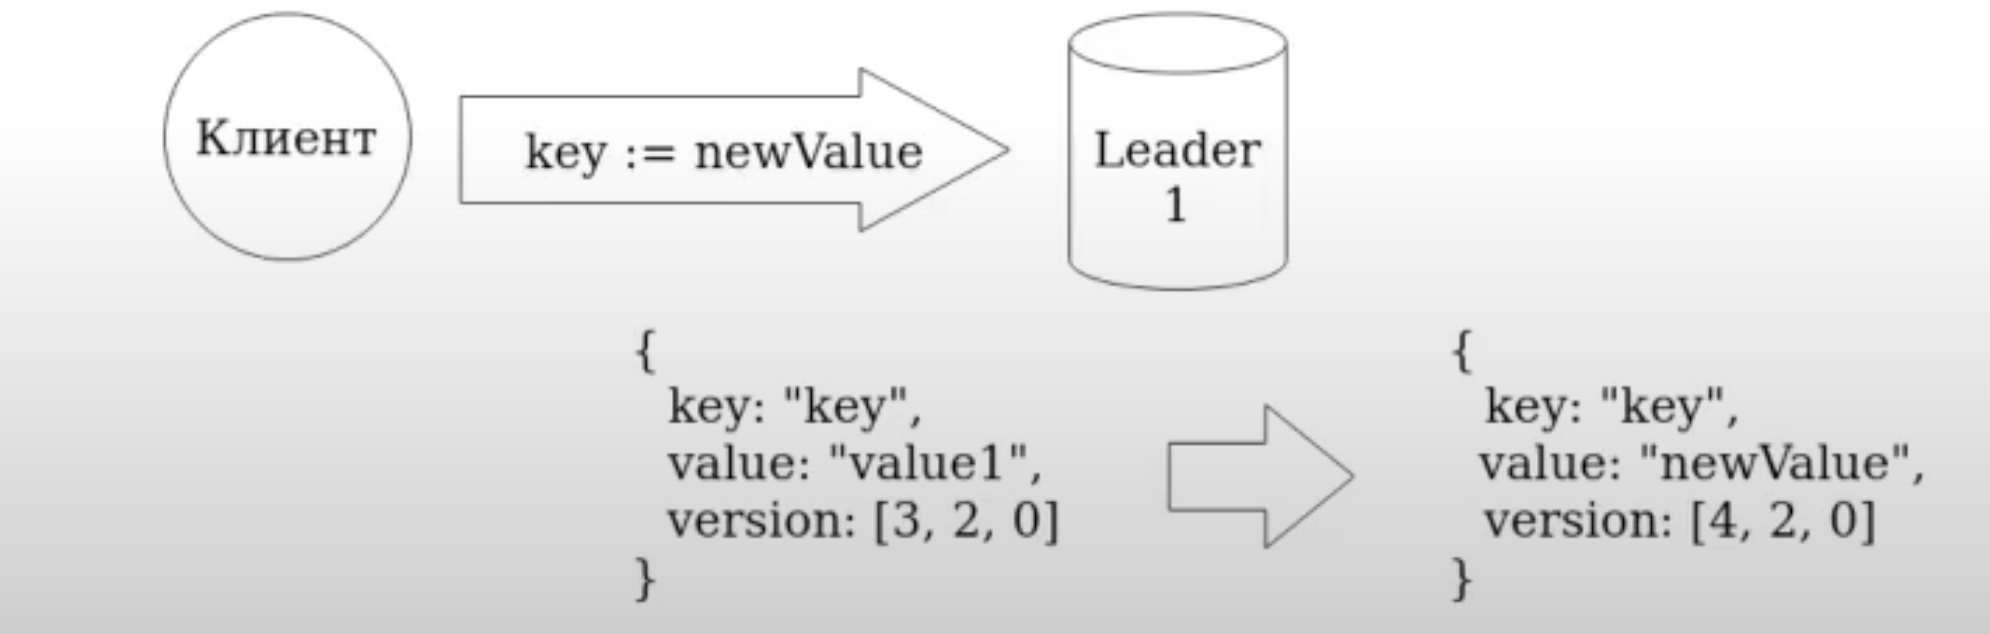
\includegraphics[scale = 0.5]{1.png}
    \caption{}
\end{figure}
\subsection{Удаление устаревших значений}
Реплики обмениваются локальными значениями вместе с версиями. \\
Если $A$ happens-before $B$, то может быть $A$ удалено. \\
$A$ happens-before $B$ - мажорирование вектора $B$ над вектором $A$.\\
\begin{figure}[h]
    \centering
    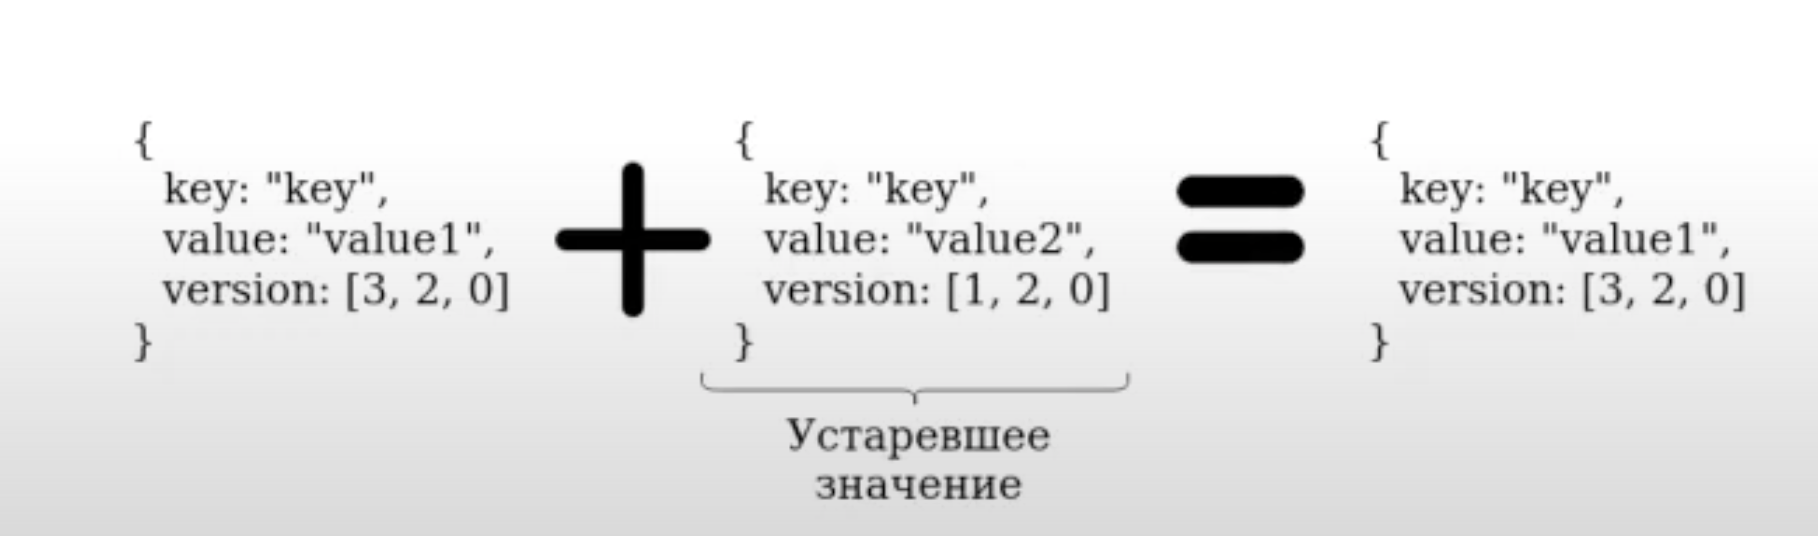
\includegraphics[scale = 0.5]{2.png}
    \caption{}
\end{figure}
\subsection{Векторные версии: параллельные обновления}
Параллельность определяется так же, как и в векторных часах. \\
Мы сами не можем определить, какое значение правильное (так как нет happens-before), тогда сохраним оба значения и пусть приложение само решит, что делать. \\
Версия получившаяся - покомпонентный максимум из двух несравнимых векторов. \\
Пример как приложение может само решать конфликты:\\
\begin{figure}[h]
    \centering
    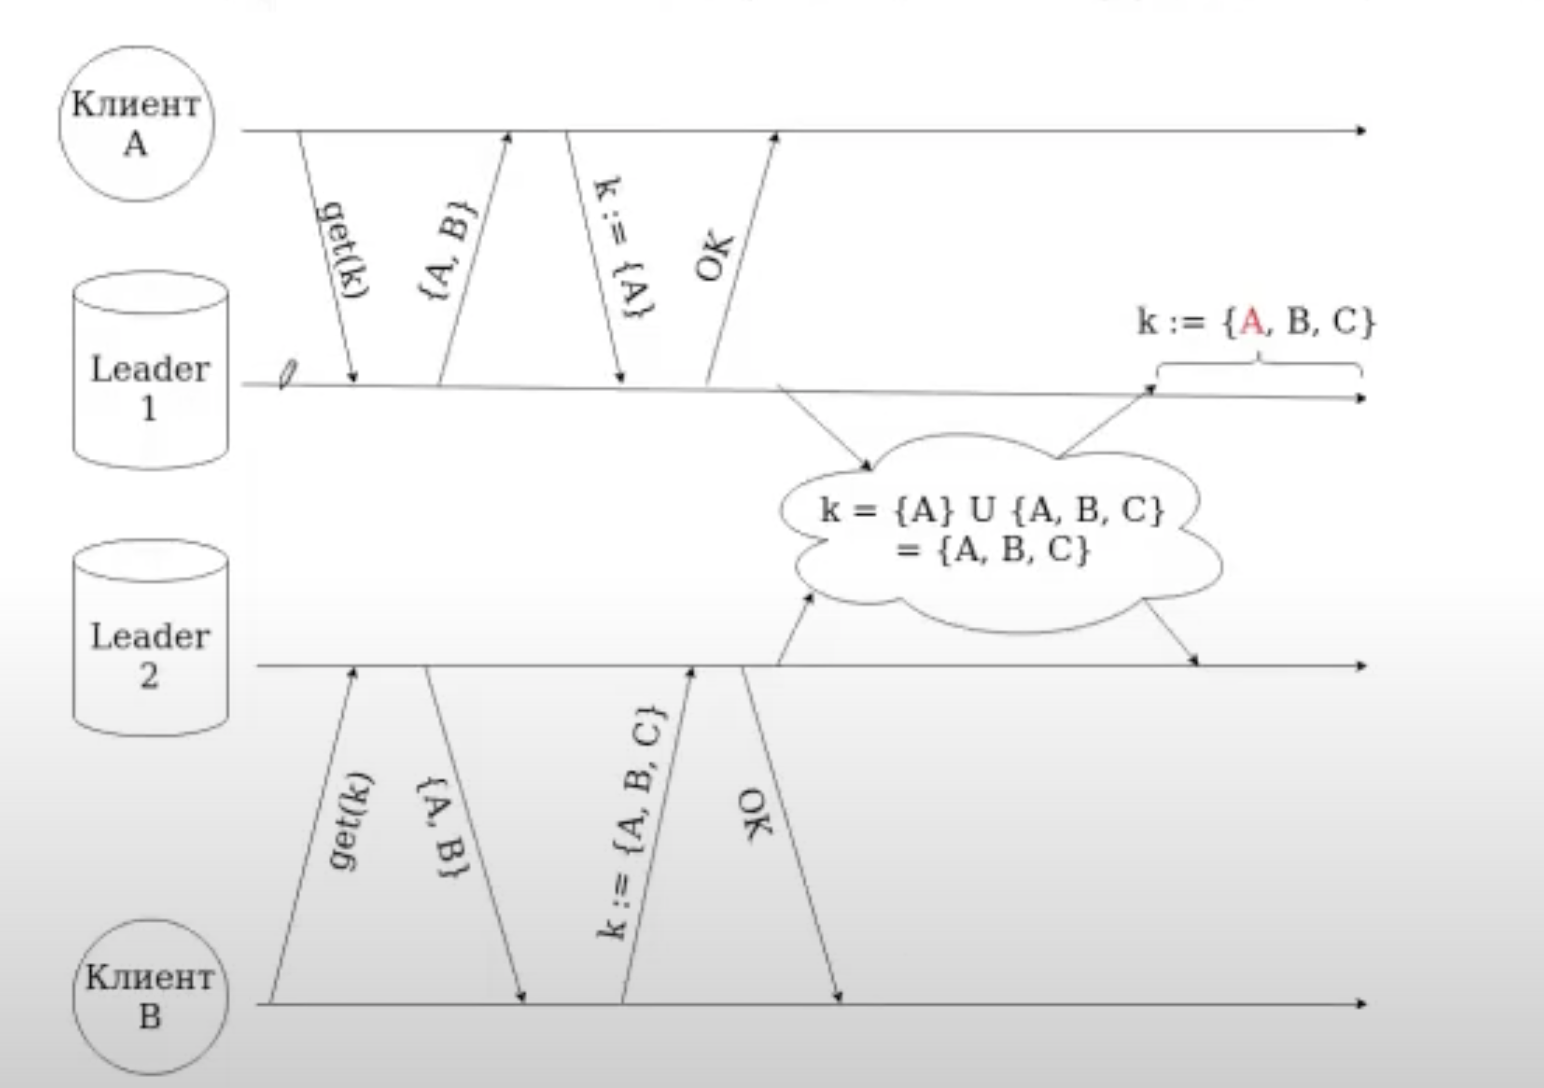
\includegraphics[scale = 0.5]{4.png}
    \caption{}
\end{figure}
Зависит от того, какие данные храним.\\
Корзина - множество объектов которые пользователь хочет купить.\\
Есть две корзины A и B (записи A и B происходят параллельно).\\
Объединяем корзины как множества.\\
"Возрождение" товаров в корзине.\\
Есть Client A, Leader 1, Leader 2, Client B.\\
Корзины отреплицированы на двух лидеров, корзина k := {A, B}.\\
Client A удаляет B на Leader 1: $k := {A}$.\\
Client B добавляет С на Leader 2: $k := {A, B, C}$.\\
Обе операции подтверждаются.\\
Записи происходили одновременно - получаем конфликт.\\
При решении конфликта - объединении множеств получаем $k = {A} \cup {A, B, C} = {A, B, C}.$\\
Можем терять только удаление из корзины, но добавление никогда не потеряем.\\
\subsection{Разрешение конфликтов при чтении}
Приложение читает данные и понимает, что версии разошлись.\\
Решает конфликт, получает итоговое значение.\\
Записывает его в базу.\\
Увеличивая локальную версию той реплики, куда новая версия будет записана.\\
Результирующему значению будут предшествовать все конфликтующие записи.\\
Результирующее значение заменит любое из них.\\
\subsection{Разрешение конфликтов при чтении на разных узлах.}
Конфликт может быть одновременно решен на нескольких узнал, но тогда получаем несравнимые вектора.\\
Вероятность такого мала, так как конфликт решается при чтении клиентом.\\
Используем детерменированное разрешение конфликтов.\\
Как обычно, либо можем сохранить два значение и дать приложению решить конфликт.\\
Мала вероятность такого конфликта, так как конфликт решается приложением при чтении, то нужно чтобы с двух разных узлов два приложения.\\ параллельно прочитали конфликтные значения, узнали что они конфликтные, решили этот конфликт и сделали параллельную запись на два разных узла.\\
\begin{figure}[h]
    \centering
    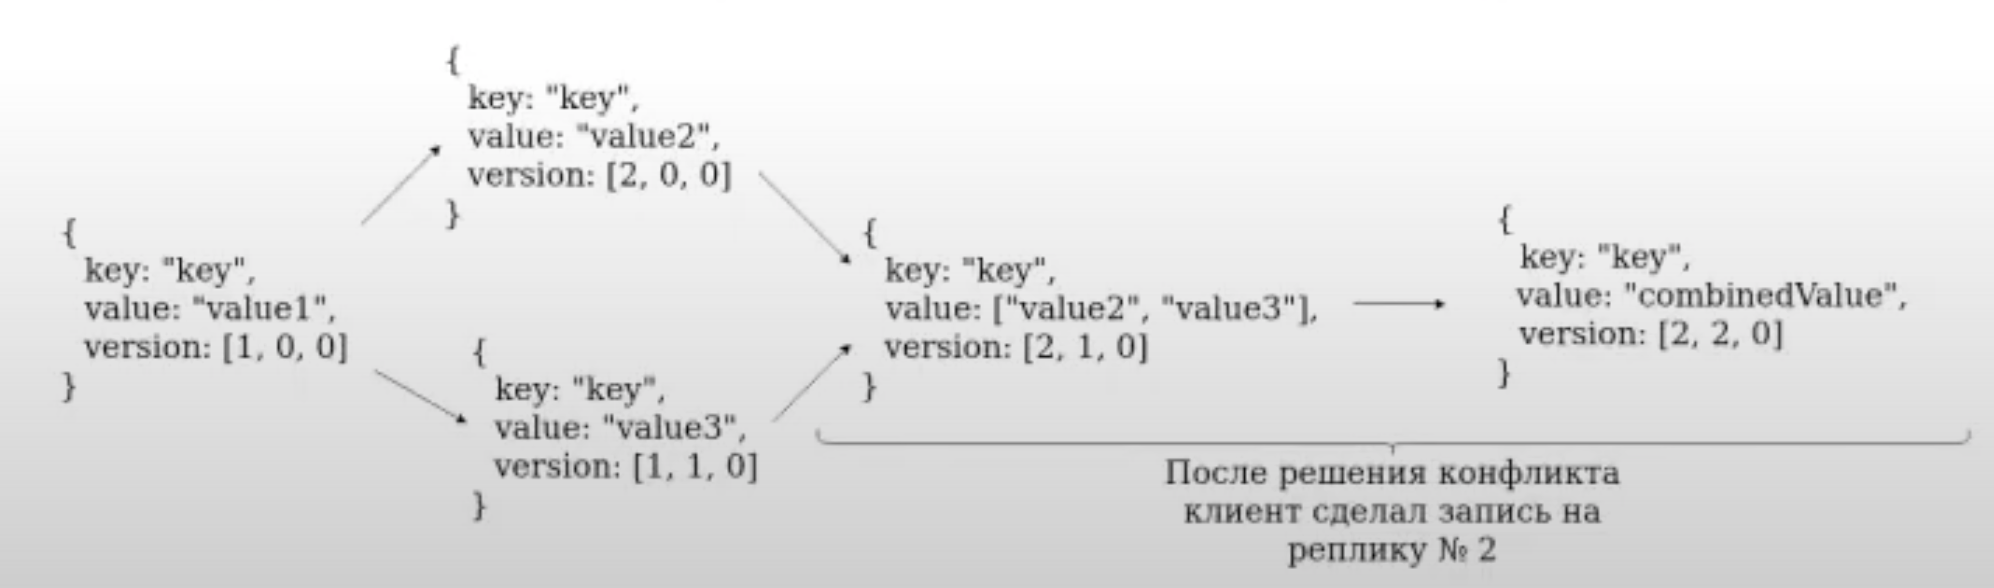
\includegraphics[scale = 0.5]{5.png}
    \caption{}
\end{figure}
\begin{figure}[h]
    \centering
    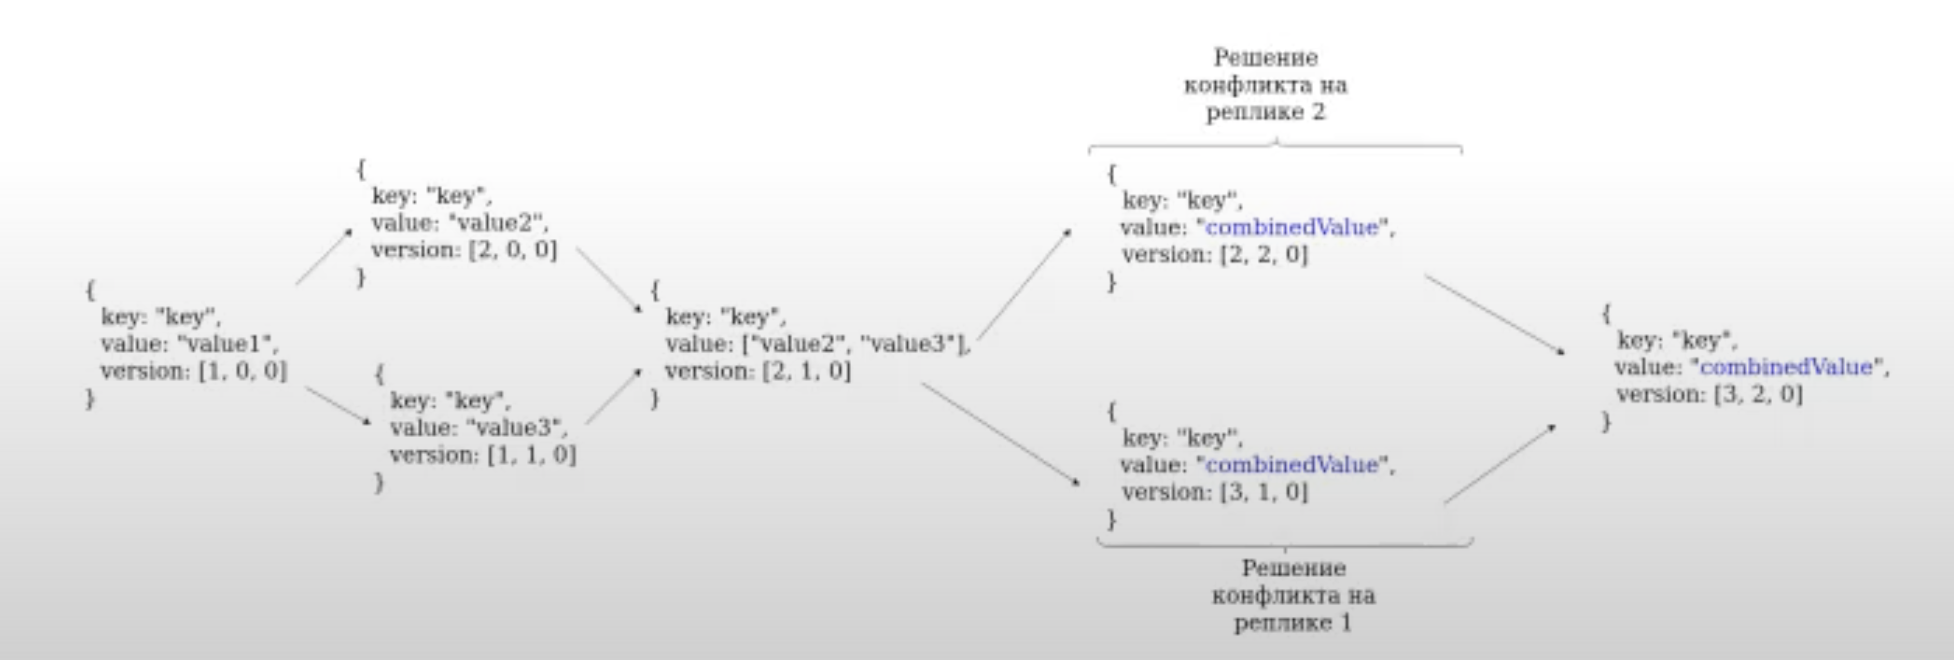
\includegraphics[scale = 0.5]{6.png}
    \caption{}
\end{figure}
Но и выйти можем по старой схеме - сохранить два конфликтных значения и дать приложению решить конфликт.
\subsection{Разрешение конфликтов при записи}
Есть конфликты, которые сама реплика может решить при получении конфликтующей версии.\\
Обычно так решаются очень простые конфликты, которые не требуют вмешательства сложной логики на стороне приложения.\\
Пример: параллельная запись в разные поля объекта.
\begin{figure}[h]
    \centering
    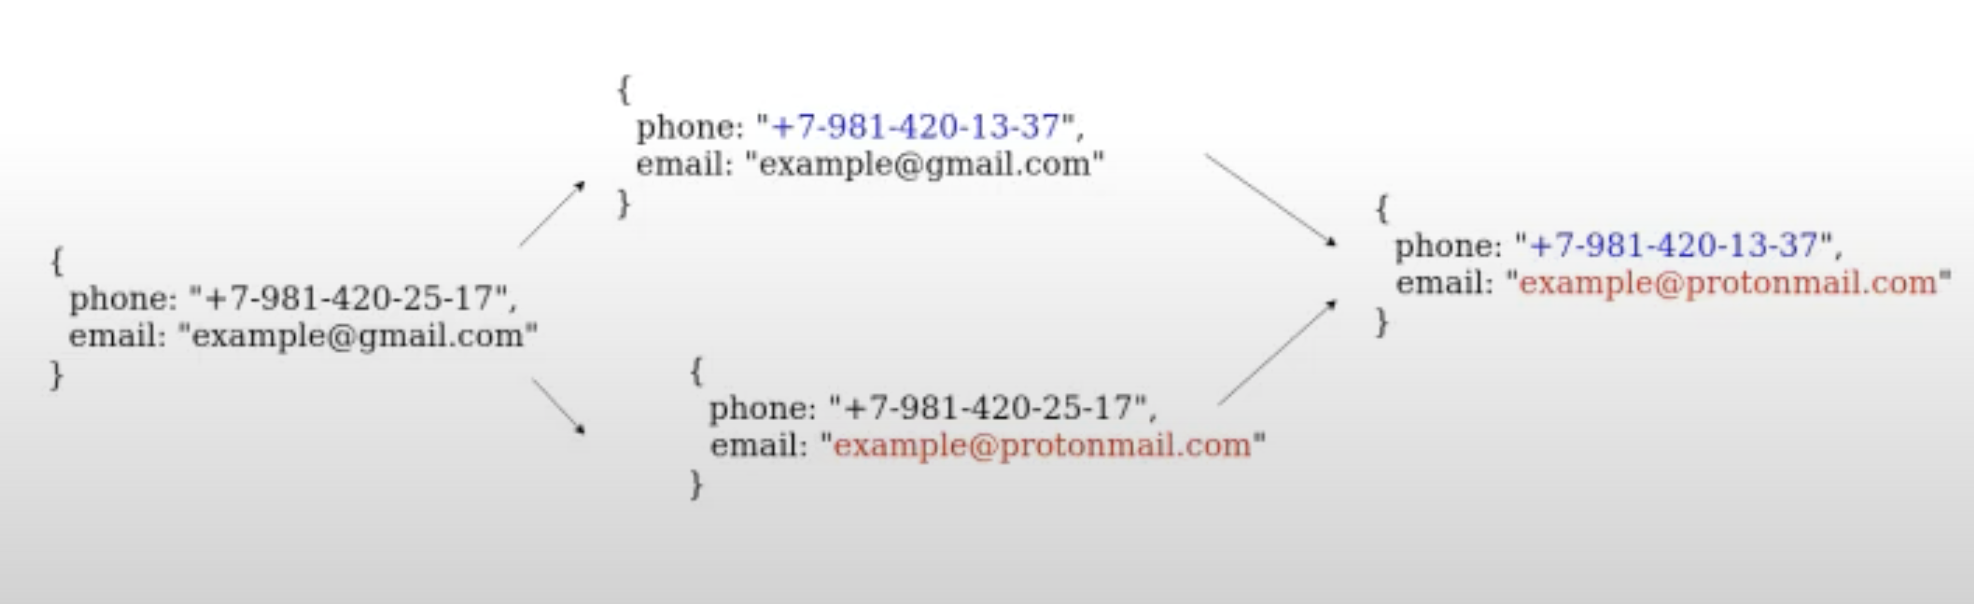
\includegraphics[scale = 0.5]{7.png}
    \caption{}
\end{figure}
\subsection{Невозможность разрешения конфликтов на уровне приложения}
Приложение не может объединить два различных электронных адреса в один корректный.\\
электронный адрес - атомарная сущность, в отличие от корзины с товарами.\\
У приложения нет возможности узнать как нужно решать конфликт - поскольку нет доступа к реальному миру.\\
В таком случае можно отдать на разрешение пользователю (так поступает git).
\begin{figure}[h]
    \centering
    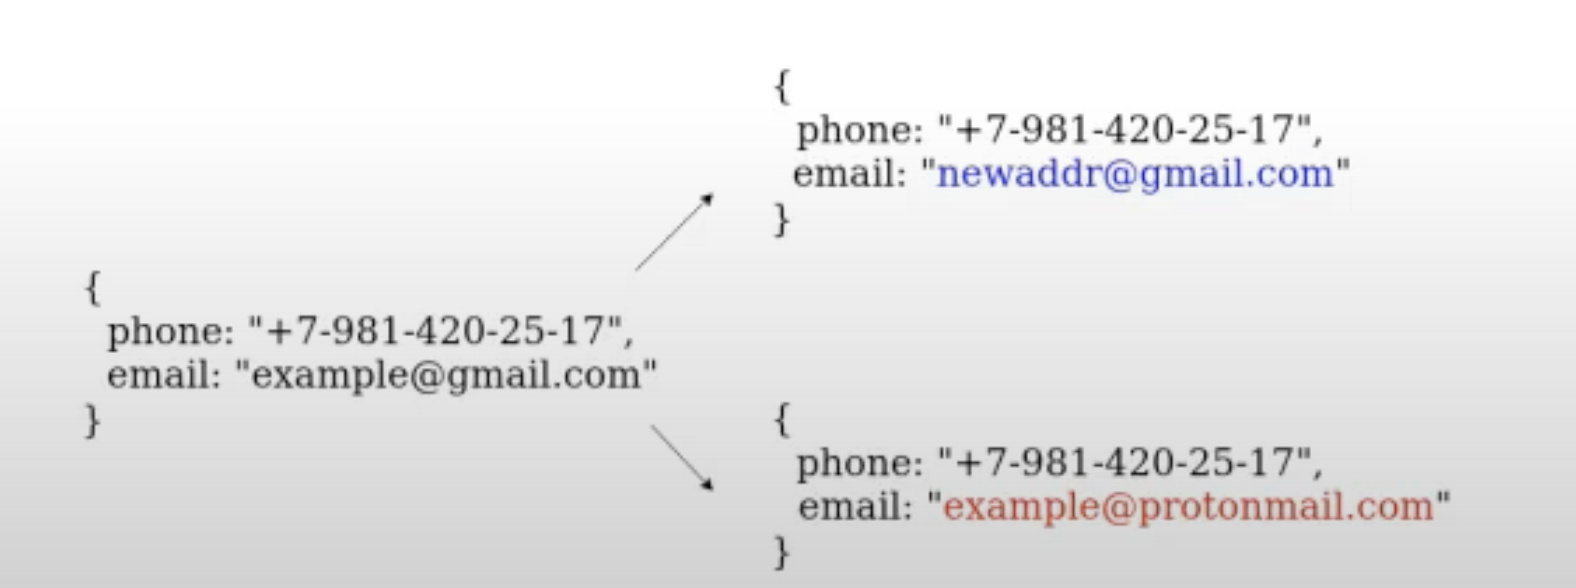
\includegraphics[scale = 0.5]{8.png}
    \caption{}    
\end{figure}
\subsection{Векторные версии: изменение состава кластера}
Вместо вектора будем хранить отображение.\\
Ключ - имя узла.\\
Значение - сколько обновлений с этого узла мы видели.\\
Если же в отображении нет нужного нам ключа - то представим, что он там есть, и значение $0$.\\
Разумно, так как мы не видели ни одного обновления с этого узла
\subsection{Векторные версии: удаление старых версий}
Мотивация - векторные часы при увеличении количества реплик и не удалении ненужных увеличиваются в размерах.\\
Хотим удалять старые значения, которые соответствуют выведенным из эксплуатации узлам.\\
Будем на каждом из узлов помнить, когда мы получали в последний раз сообщение от каждой из реплик.\\
Из векторных часов будет удалять ключ, который соответствует реплике, от которой дольше всего не получали сообщений, так как с наибольшей вероятностью эта реплика мертвая.\\
Есть возможность потерять отношение happens-before.\\
\begin{figure}[h]
    \centering
    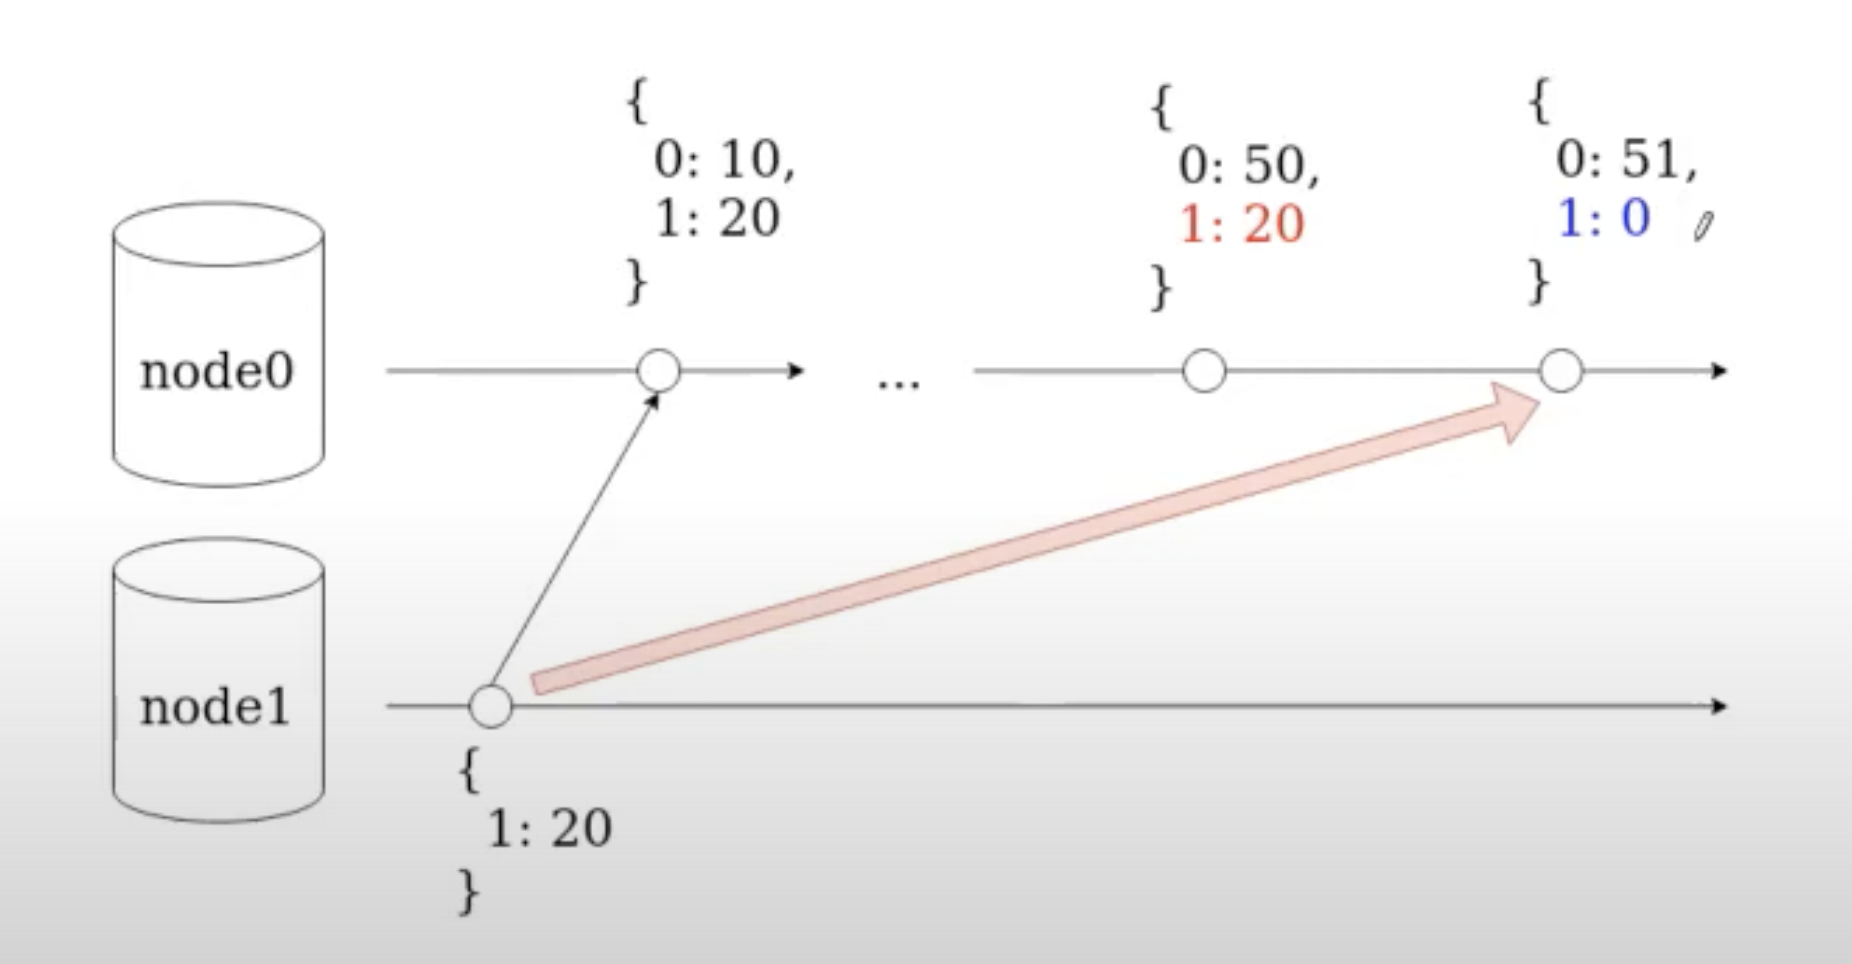
\includegraphics[scale = 0.5]{9.png}
    \caption{}
\end{figure}
Если у нас есть метод объединения кофликтующих версий - просто объединим эти версии.\\
Вместо удаления старой версии.
